\everymath{\displaystyle}
\documentclass{beamer}
% \documentclass[handout]{beamer}

%\usepackage[pdftex]{color,graphicx}
\usepackage{amsmath,amssymb,amsfonts}

\mode<presentation>
{
  % \usetheme{Darmstadt}
  % \usetheme[hideothersubsections]{Hannover}
  % \usetheme[hideothersubsections]{Goettingen}
  \usetheme[hideothersubsections, right]{Berkeley}

  \usecolortheme{seahorse}
  % \usecolortheme{dolphin}
  \usecolortheme{rose}
  % \usecolortheme{orchid}

  \useinnertheme[shadow]{rounded}

  \setbeamercovered{transparent}
  % or whatever (possibly just delete it)
}

\mode<handout>{
  \setbeamercolor{background canvas}{bg=black!5}
  \usepackage{pgfpages}
  \pgfpagesuselayout{4 on 1}[a4paper,border shrink=5mm, landscape]
}

\usepackage[brazilian]{babel}
% or whatever

% \usepackage[latin1]{inputenc}
\usepackage[utf8]{inputenc}
% or whatever

\usepackage{times}
%\usepackage[T1]{fontenc}
% Or whatever. Note that the encoding and the font should match. If T1
% does not look nice, try deleting the line with the fontenc.


\title[Estatística na Pesquisa] % (optional, use only with long paper titles)
{A Importância da Análise Estatística na Pesquisa}

\subtitle
{} % (optional)

\author%[] % (optional, use only with lots of authors)
{Felipe Figueiredo}% \and S.~Another\inst{2}}
% - Use the \inst{?} command only if the authors have different
%   affiliation.

\institute[INTO] % (optional, but mostly needed)
{Mestrado Profissional em Ciências Aplicadas ao Sistema Musculoesquelético\\
Instituto Nacional de Traumatologia e Ortopedia Jamil Haddad
}
  % \inst{1}%
  % Department of Computer Science\\
  % University of Somewhere
  % \and
  % \inst{2}%
  % Department of Theoretical Philosophy\\
  % University of Elsewhere}
% - Use the \inst command only if there are several affiliations.
% - Keep it simple, no one is interested in your street address.

\date%[] % (optional)
{18/11/2016}

% \subject{Talks}
% This is only inserted into the PDF information catalog. Can be left
% out. 



% If you have a file called "university-logo-filename.xxx", where xxx
% is a graphic format that can be processed by latex or pdflatex,
% resp., then you can add a logo as follows:

\pgfdeclareimage[height=1.6cm]{university-logo}{logo}
\logo{\pgfuseimage{university-logo}}



% Delete this, if you do not want the table of contents to pop up at
% the beginning of each subsection:
\AtBeginSubsection[]
%\AtBeginSection[]
{
  \begin{frame}<beamer>{Sumário}
    \tableofcontents[currentsection,currentsubsection]
  \end{frame}
}


% If you wish to uncover everything in a step-wise fashion, uncomment
% the following command: 

% \beamerdefaultoverlayspecification{<+->}


\begin{document}

\begin{frame}
  \titlepage
\end{frame}

% \begin{frame}{Sumário}
%   \tableofcontents
%   % You might wish to add the option [pausesections]
% \end{frame}


%% Template
% \section{}

% \subsection{}

% \begin{frame}{}
%   \begin{itemize}
%   \item 
%   \end{itemize}
% \end{frame}

% \begin{frame}
%   \begin{columns}
%     \begin{column}{5cm}
%     \end{column}
%     \begin{column}{5cm}
%     \end{column}
%   \end{columns}
% \end{frame}

% \begin{frame}{}
%   \includegraphics[height=0.4\textheight]{file1}
%   \includegraphics[height=0.4\textheight]{file2}
%   \includegraphics[height=0.4\textheight]{file3}
%   \begin{figure}
%     \caption{}
%   \end{figure}
% \end{frame}

% \begin{frame}{}
%   \begin{definition}
%   \end{definition}
%   \begin{example}
%   \end{example}
%   \begin{block}{Exercício}
%   \end{block}
% \end{frame}

\begin{frame}
  \begin{center}
    {\bf O que é e para que serve}
  \end{center}
\end{frame}

\begin{frame}
  \begin{center}
    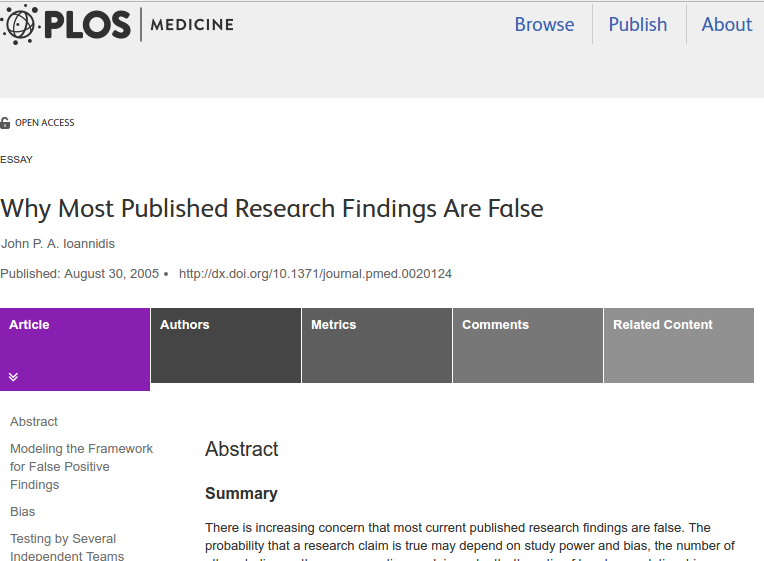
\includegraphics[height=.75\textheight]{Imagens/Ioannidis}

    \bigskip
    Ioannidis (2005)
  \end{center}
\end{frame}

\begin{frame}{}
  \begin{block}{}
    Se você torturar os dados o suficiente, eles confessarão o que você quiser.
  \end{block}
\hfill Ronald H. Coase (1982)
\end{frame}

\begin{frame}
  \begin{center}
    {\bf Perguntas frequentes}
  \end{center}
\end{frame}

\begin{frame}
  \begin{center}
    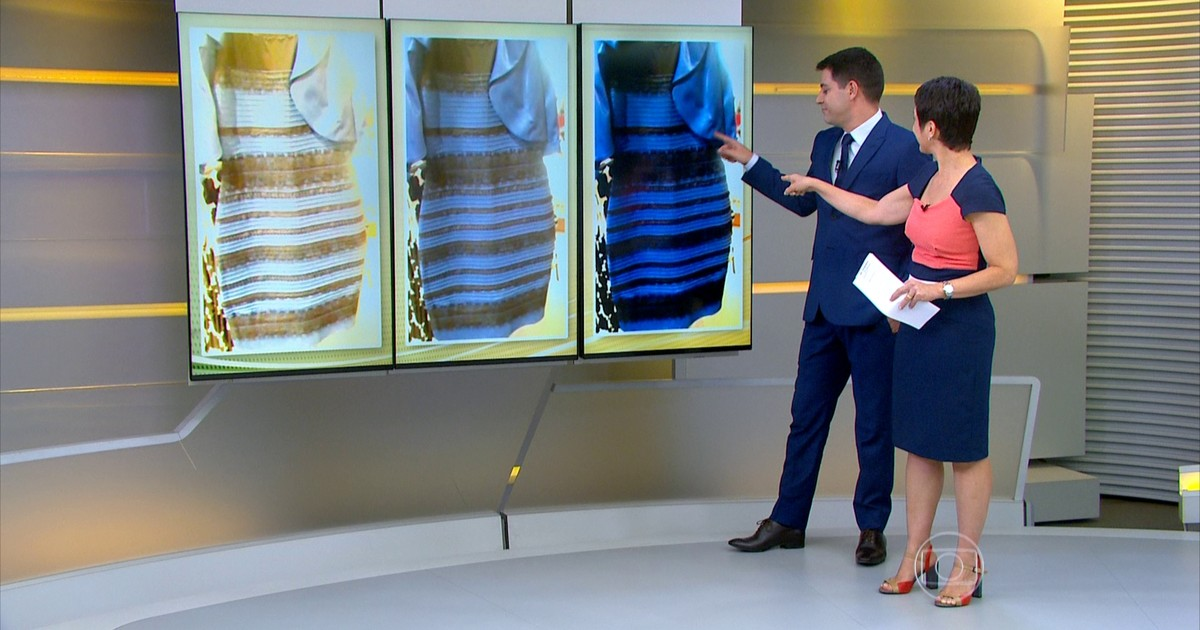
\includegraphics[width=\textwidth]{Imagens/pergunta1}

    Qual é a cor deste vestido?
  \end{center}
\end{frame}

\begin{frame}
  \begin{center}
    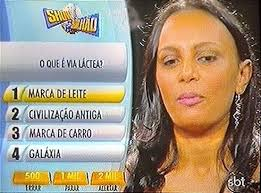
\includegraphics[width=.7\textwidth]{Imagens/pergunta2}
  \end{center}
\end{frame}

\begin{frame}
  \begin{block}{A pergunta mais frequente}
    Tenho estes dados... o que posso descobrir com eles?
  \end{block}
\end{frame}

\begin{frame}
  \begin{block}{}
    Chamar o estatístico depois que o experimento está concluído é chamá-lo para um exame post-mortem...

\bigskip
\uncover<2>{talvez ele possa lhe dizer de que o experimento morreu.}
  \end{block}
\hfill Sir Ronald Fisher (1938)
\end{frame}

\begin{frame}
  \begin{center}
    {\bf Reproducibilidade}
  \end{center}
\end{frame}

\begin{frame}
  1500 cientistas responderam a uma pesquisa sobre reproducibilidade (Nature, 2016)

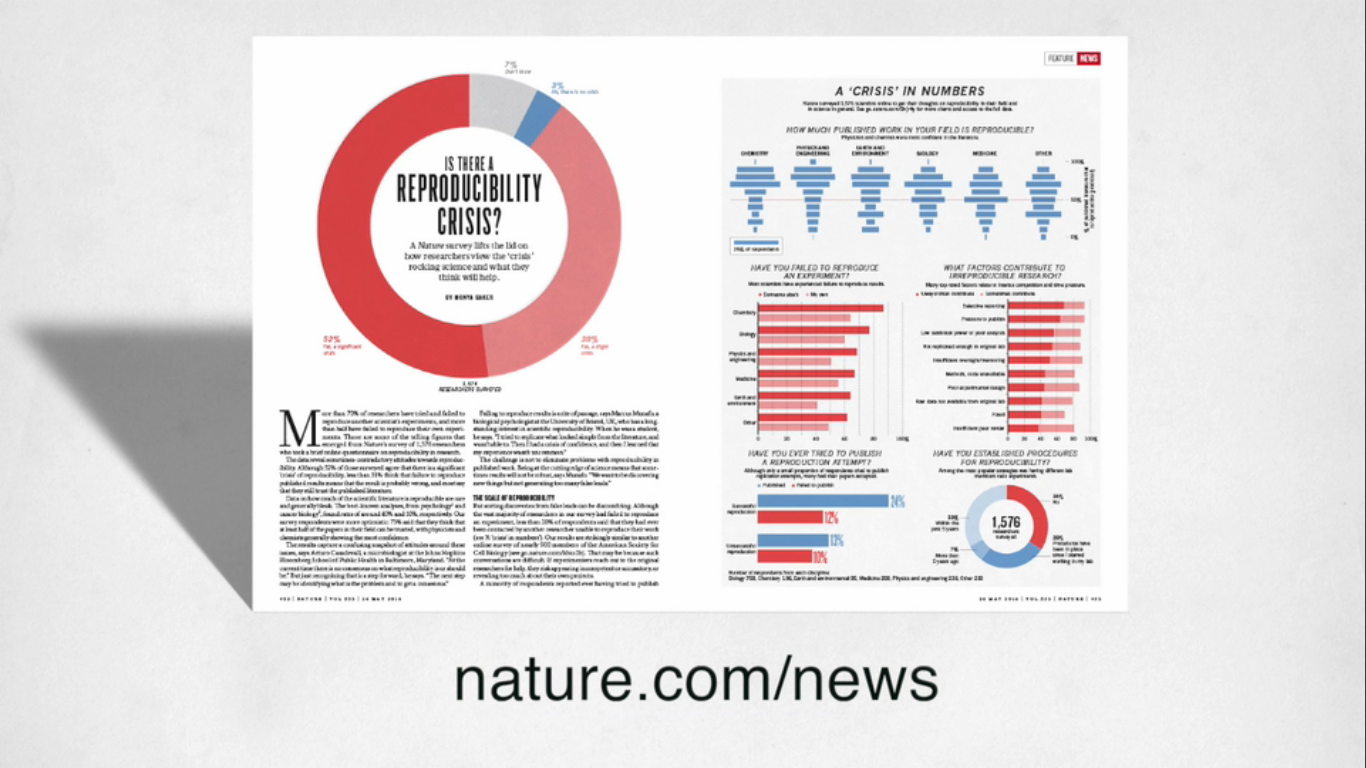
\includegraphics[width=\textwidth]{Imagens/reprod-nature3}
\end{frame}

\begin{frame}
  \begin{center}

    \begin{columns}
      \begin{column}{5cm}
        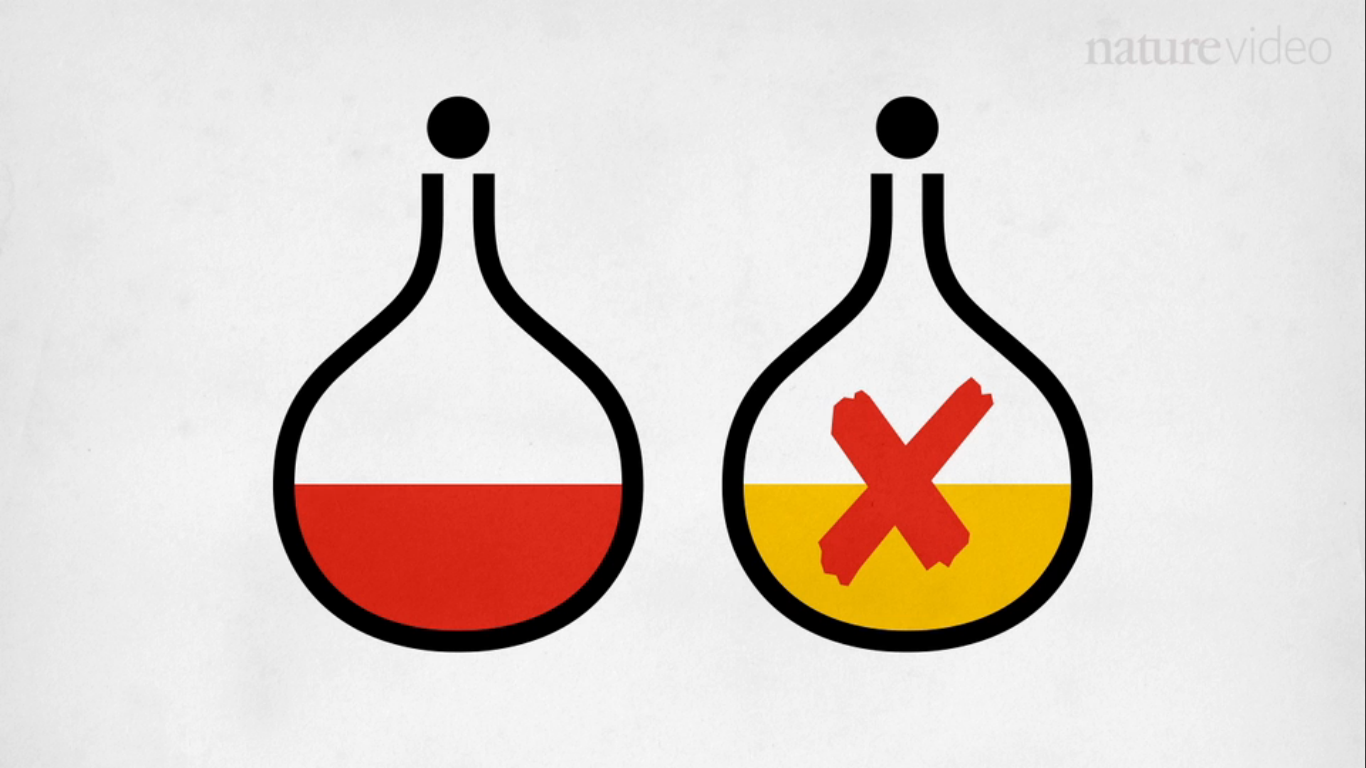
\includegraphics[width=\textwidth]{Imagens/reprod-nature1}

$>70\%$ não conseguiram reproduzir algum experimento de algum outro grupo
      \end{column}
      \begin{column}{5cm}
        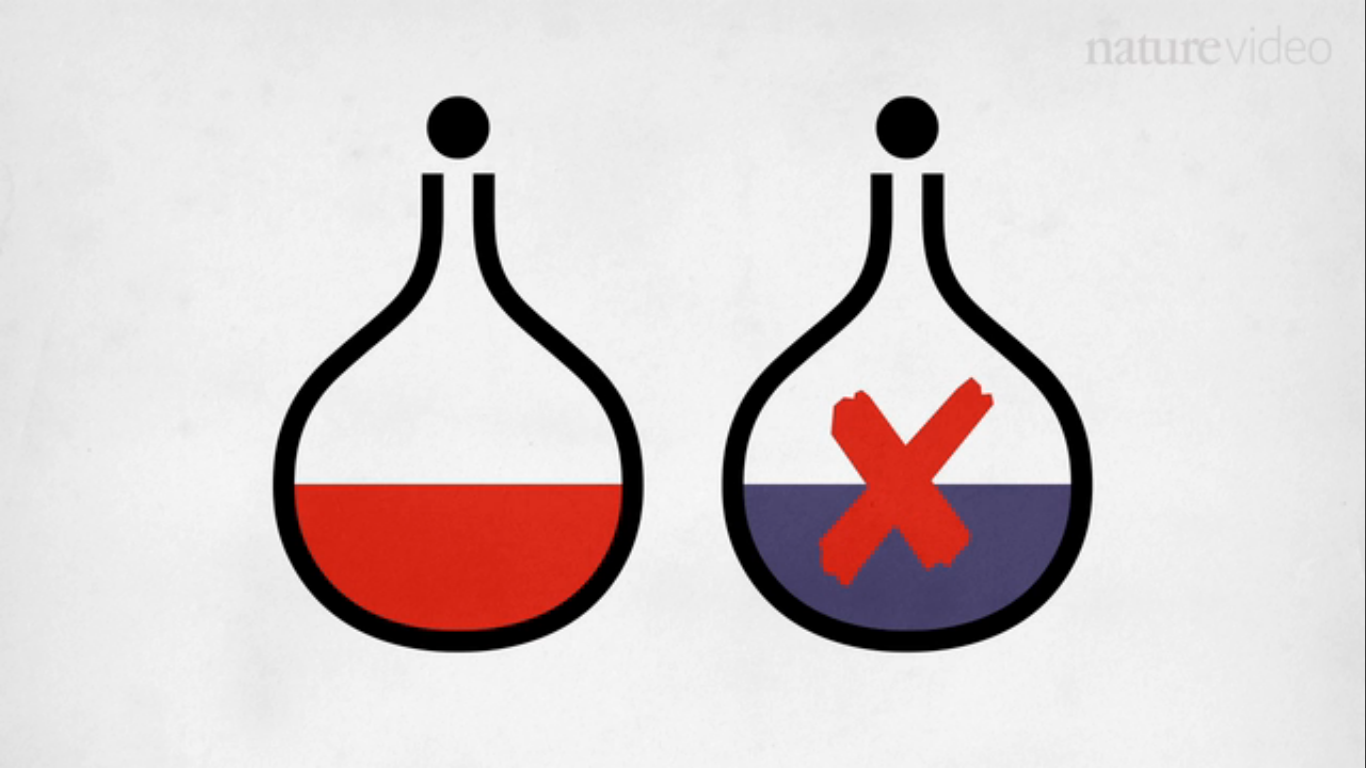
\includegraphics[width=\textwidth]{Imagens/reprod-nature2}

$>50\%$ não conseguiram reproduzir algum experimento de seu próprio grupo
      \end{column}
    \end{columns}
  \end{center}
\end{frame}

\begin{frame}
  \begin{block}{Principais causas?}
    \begin{itemize}
    \item Relatos seletivos
    \item Pressão para publicar
    \end{itemize}
  \end{block}
\end{frame}

\begin{frame}{Métodos mal documentados...}
  \begin{center}
    
\includegraphics[width=\textwidth]{Imagens/Vasilevsky}

  \end{center}
\end{frame}

\begin{frame}{... podem levar a erros metodológicos}
  \begin{center}
    
\includegraphics[width=\textwidth]{Imagens/Baggerly}
  \end{center}
\end{frame}

\begin{frame}
  \begin{block}{Como melhorar a reproducibilidade?}
    De acordo com o estudo da Nature
    \begin{itemize}
    \item Melhor compreensão de Estatística
    \item Desenhos experimentais mais robustos
    \item Melhor supervisão/orientação
    \end{itemize}
  \end{block}
\end{frame}

\begin{frame}
  \begin{block}{}
    A combinação de um punhado de dados e um desejo ardente por uma resposta não garante que uma resposta razoável pode ser extraída de um conjunto de dados
  \end{block}
\hfill John W. Tukey (1986)
\end{frame}

\end{document}
